To understand how machine facial detection works, let us try to reflect on what humans \textit{actually} do to identify faces: their sensory, visual perceptors - the eyes - capture an image and send it to the brain. The brain, in turn, translates that image into a \textit{thought}, an abstract representation, in which it searches for the existence of features, such as noses, eyes, mouths, hairlines, all being, essentially, high contrast points on a generally oval-shaped background (the face), which itself stands in contrast to a differently-colored background. In similar fashion, neural-network powered face detection takes a digital image, translates it into a representation that is understandable to computers via convolution, then looks for features and identifies them inside that new representation. The more features are present, the higher the confidence our ML-system can express towards the existence of a face in that given input. \par
If we were to sum up Machine Learning facial detection in one sentence, it would sound something similar to this: a computer translates a picture into a mathematical model, wherein it searches for patterns, which in turn confirm or infirm the existence of a face in a particular region of that specific given picture. \par

\section{Classical Approaches for Face Detection} 
The methods presented below do not use neural networks for achieving their goal. They are based on methods from some years ago, which belong to what could be labelled as \textit{classical} Machine Learning instead. \cite{classic_ml_quora}
\subsection{Viola-Jones}
With the advent of point-and-shoot digital cameras in the early 2000's, the manufacturers needed a simple, low-overhead, real-time procedure of identifying faces in an image, that could run on the constrained hardware of a digital camera. Thus, the Viola-Jones procedure (named after its authors) was created. The initial image classifier consists of a 38-layer cascaded network architecture. It was based, in essence, on a set of classifiers, which, would have offered poor accuracy as individual units, but, combined, offered greatly improved detection. \par 
The Viola-Jones classifier was trained on around 4900 face images and 9600 non-face, negatives. It achieved an accuracy of around 95\%, and can process images at up to 15 frames per second. \cite{viola_jones_1} The face detector was then developed and expanded into into a general object classifier by the authors. Although it uses a similar model architecture, the object classifier does not take direct images as inputs anymore, but feature maps instead. \cite{viola_jones_2} \par
Feature maps are, esentially, some measurable form of a property of, in our case, an image, or at least of some part of one image. \cite{pat_rec_springer} In this case, it is edges and contrast differences that let us identify the face as an object inside an image. 
\subsection{Histogram of Oriented Gradients}
Another widely-used procedure for classical image classification is Histogram of Oriented Gradients (HOG). This procedure essentially divides an image up into separate regions based on contrast. Inside these regions, we calculate the gradient - rate of change - in order to determine patterns. The concatenation of these features is saved as a new representation, which indicates the contents as belonging to a certain class, which can be identifiable. The main advantage of HOG is that its accuracy only depends on geometric shapes, but not on chromatic or contrast differences, which would influence the performance of older methods. Images used for HOG are normalized and their dynamic range reduced to further improve accuracy. \cite{HOG_humans} Mathematically, a HOG detector identifies \textit{oriented Haar wavelets} \cite{haar_1910}, which are brief oscillations, starting slightly above zero (as absolute values) and soon dropping back to very close to zero again. Picking up on these \textit{signals} is the main mathematical principle HOG depends on. HOG is often used for general shape detectors, where we don't want to use neural networks.
\subsection{Support Vector Machines}
Finally, let us look into SVM's, which are a more sophisticated category of Machine Learning technique that can be used for facial detection. Support vector machines are supervised learning systems, which can separate samples into different planes, and therefore determine which class different objects belong to. A visual representation can be seen in \textit{Figure \ref{fig:svm}}. \cite{svm}
\begin{figure}
    \centering
    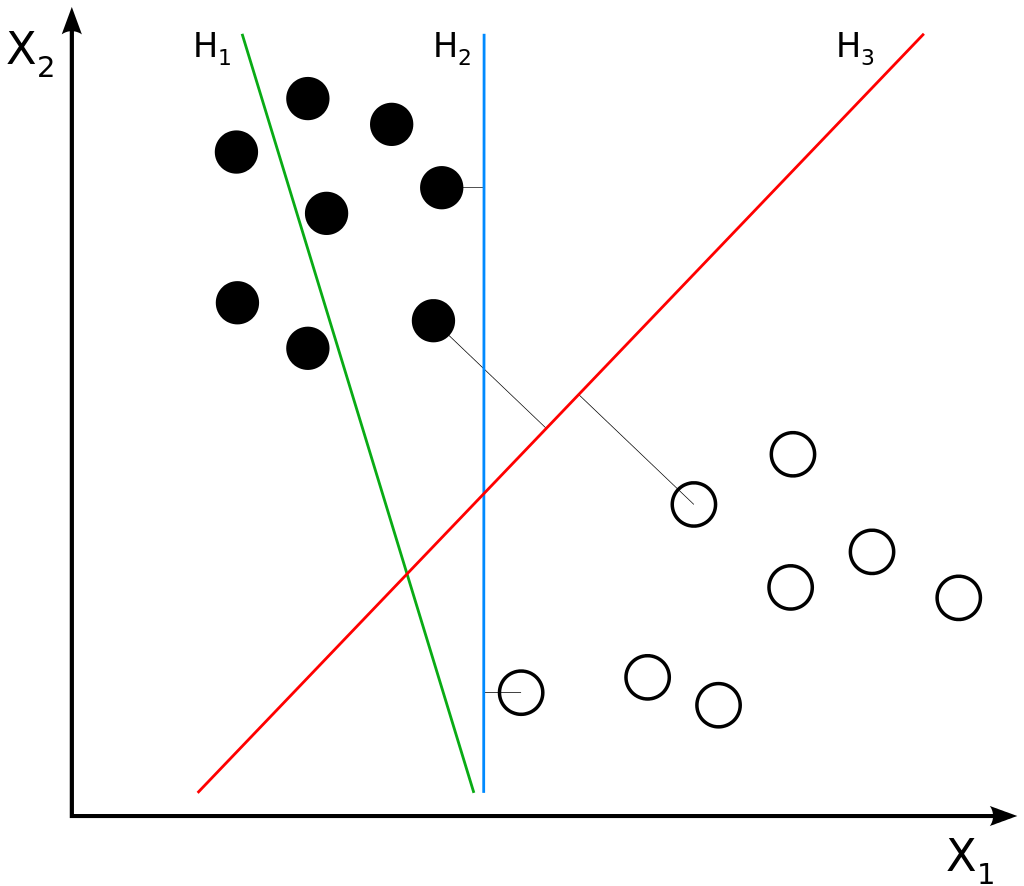
\includegraphics[width = 10 cm]{images/Svm_separating_hyperplanes_(SVG).svg.png}
    \caption{Visual representation of a Support Vector Machine. Source: \cite{svm_pic}}
    \label{fig:svm}
\end{figure}

\section{Face Detection with Convolutional Neural Network Classifiers}
To understand how face detection with convolutional neural networks works, we need to firstly define \textit{binary classifiers}. Binary classification is the process of assigning one of several different classes to an object, according to a set of rules. In order to find these rules, a neural network needs \textit{labelled} training data, from which it can extract features, and then \textit{learn} which family of objects those attributes belong to. As such, we can formulate the problem of facial detection with convolutional neural networks as a 4-step procedure.
\begin{enumerate}
    \item Designing a model architecture
    \item Compiling training data
    \item Training a classifier, compression and optimization
    \item Performing inference
\end{enumerate}
The first 3 steps will be executed \textit{a priori}, on a separate, more powerful computer. The final step requires us to use an embedded, edge device. We will address the first 3 steps in this chapter, and the final step in chapters 5 and 6. 

\section{Designing a Convolutional Neural Network Model Architecture}
For the building of a neural network model architecture, several formerly designed models, from literature, were analyzed to determine their fitness for TinyFace. An overview of some of the most prominent examples the author has experimented with, are listed below.
\begin{enumerate}
    \item SqueezeNet \cite{squeezent_paper}
    \item DarkNet \cite{tiny_darknet}
    \item LeNet \cite{lenet_1}
    \item VGG \cite{vgg_paper}
\end{enumerate}
The author has built a Python-based framework, on which many different combinations of datasets and model architectures were trained and tested, with different hyperparameters. The results of this process will be discussed in Chapter 5. \par
A more advanced neural network model architecture, developed by Google and available open-source, has also been considered. It is called FaceNet, and it was primarily designed for facial recognition, since it can \textit{very} accurately identify facial features of individuals and tell apart one person from another with over 90\% accuracy after having trained on just 10 pictures of that person. FaceNet therefore is not only capable of face detection, but also advanced one-to-many facial recognition, and this puts it outside the scope of this project, or the performance of embedded hardware in general. \cite{facenetseminal_paper} \par
As we can see in \textit{Table \ref{tab:model_archs}}, out of the several investigated model architectures, the best TinyFace performance has been achieved by an optimized version of SqueezeNet, the size of which the author has reduced by using TF-Lite quantization and compression.
\subfile{tables/models}

\section{Gathering Data for Training Neural Networks}
As we have repeatedly seen, gathering relevant and properly selected data for training and validation, which presents high \textit{statistical variance}, is of paramount importance to achieving high accuracy for our final model, when performing inference on real-world data.  In the following sub-sections, we will discuss an end-to-end approach for compiling datasets of images of actors' faces, filtering the data, pre-processing the images to the desired dimension and color channels, and finally exporting them into a format that is appropriate for model training.
\subsection{Compiling a Dataset}
Dataset generation is a task that is often best accomplished with automation. Having resolved to also generate our own data for training, a Python scripted tool for web-scraping and image processing was built. \par
In essence, the tool can search Google and IMDb by actor names, compile a list of links of images of the actors by using Selenium \cite{selenium_website} and BeautifulSoup, then download and save the images from those links. Afterwards, the tool automatically detects the faces in those images with OpenCV, crops them out with a \textit{randomized} padding border to increase variance of background, then saves those faces to the desired output shape given by the user. It can save the images as either 8-bit RGB or grayscale. \par
Using this tool, several training datasets were compiled, and the above named models were trained using this training data.\par
The finally compiled dataset consists of two categories of labelled pictures: firstly, images of faces, then, secondly, images of random backgrounds extracted from pictures, which are used as so-called \textit{negatives}. The reason we need this second class of pictures is because a binary classification tool needs, as its name suggests, exactly two classes to fit objects into.
\subfile{tables/datasets}
\subsection{Image data processing}
To process the downloaded pictures into a format suitable for face detection, the above presented tool has the ability to, firstly, filter out the faces from the larger downloaded images, than to save those faces as individual pictures, with a border padding that is randomly defined - to help with versatility - then save them, either as color or grayscale pictures, and to a desired dimension. Furthermore, we can define custom padding borders for images, including a randomizer that ensures we always set the face slightly off-center.

\section{Training the Model}
Having now seen how a dataset can be compiled, let us look into what training could be like. 
\subsection{Discussing Datasets}
We start off with \textit{numpy} arrays of data. These are usually represented as having 4 dimensions in memory, and, therefore, a shape of \textit{n:x:y:c}. Some examples of datasets that were used by the author during training, as well as the shape of their contents can be seen in \textit{Table \ref{tab:numpy_training_shape}}. The best performance was achieved using \textit{Own Dataset 3}. A number 3 for Color Channels represents RGB images, a 1 represents grayscale images. For each color channel, we then have a \textit{0-255} value, representing its respective color as an 8-bit number. We can calculate the total, uncompressed, size of the training data array by multiplying the numbers on every row. \par
Having these rough representations for dataset size, let us now look at actually using this training data.
\subfile{figures/sqnet_tr}

\subsection{Tuning Hyperparameters}
As we have seen in Chapter 2, hyperparameters such as training batch sizes, number of epochs, training data dimensions, randomness and variance or the amount of shuffling in the dataset, can have a relatively large impact on the final performance of the neural network, when it comes to inference. \par
We have empirically determined that, in order to avoid over- and underfitting, and achieve acceptable accuracy and performance during inference with actual faces, grabbed real-time from a camera, we need around 5 epochs of training, with batch sizes ranging from 16 to 128 samples. Such a low number of epochs has been determined to be necessary to avoid overfitting. A total dataset size of 40,000 labelled samples - out of which 15,000 will be faces and 25,000 will be non-face negatives - with dimensions of \textit{100*100*1}, grayscales therefore, shuffled, and with randomized borders around the faces, have been providing acceptable real-world performance. \par
Examples of the training process of a SqueezeNet-class model can be be seen in \textit{Figure \ref{fig:squeezenet_30ep_10bat_lfw_full}} - a full size model and \textit{Figure \ref{fig:squeezenet_30ep_10bat_lfw_tfl}}, in which our model is being quantized and compressed during training.

\section{Inference and Performance Evaluation}
For testing the performance of the compiled and trained models, we are using a Python-based TensorFlow Lite model interpreter, which we are feeding images as inputs, to perform inference on. It parses the image arrays through the weights tensor, and outputs confidence percentages as to whether the objects in the images belong to certain classes. The model interpreter can take input images from 2 sources: either from image files, or directly grab frames from the webcam. This application can run on any system which has Python installed and can very quickly help us validate the real-world performance of a model. It will be presented in more detail in Chapter 5. \par
Having looked into face detection, from both a historical, pre-Convolutional Neural Network, perspective, as well as at modern CNN-powered technologies, and having the knowledge to train, compile and evaluate Neural Network models, then to translate full-size tensors into compressed, embedded-sized, packages, we can now finally enter the next chapter: the implementation of \textit{TinyFace}.
